\documentclass[12pt,twoside,a4paper]{report}
\usepackage{tikz}
\renewcommand\thesection{\arabic{section}}
\title{CMPT 843 Project}
\author{Marten Heidemeyer\\mheideme@sfu.ca}
\date{\today}
\usepackage[font=small,labelfont=bf]{caption}
\begin{document}
\maketitle
\section{Motivation and Application Background}
0.5 pages
My own application of the method. Also talk about the extra work I did (reproducing the experiments and adding extra measures).
\section{Background}
Triangles can be a more or less important structure of a graph. If many nodes are reachable from those nodes that are forming a triangle this triangle is important to connect the remaining nodes. In this case the triangle is serving as a hub for the nodes around it. Removing the nodes that form the triangle or the edges between them would disconnect a large part of the graph. The importance of one triangle can be calculated as the number of nodes that are adjacent to it. Let this sum be defined as the \textit{connectivity} of a triangle. Figure 1 shows a graph with three triangles with \textit{connectivity} 15, 14 and 10. The average \textit{connectivity} of triangles in this graph is $\frac{15+14+10}{3}=13$. If we want to find the average \textit{connectivity} of triangles in a large scale graph it makes sense to sample a number of triangles and observe the \textit{connectivity} of the sampled triangles. In this report I document the application of the \textit{Neighborhood Sampling} method as introduced in the paper "Counting and Sampling Triangles from a Graph Stream" to estimate the average connectivity of the overall population of triangles in the graph. Here I will limit the experiments to triangles for which the adjacent nodes are distributed evenly across the three nodes of the triangle as in the graph of Figure 1.
 
\begin{figure}
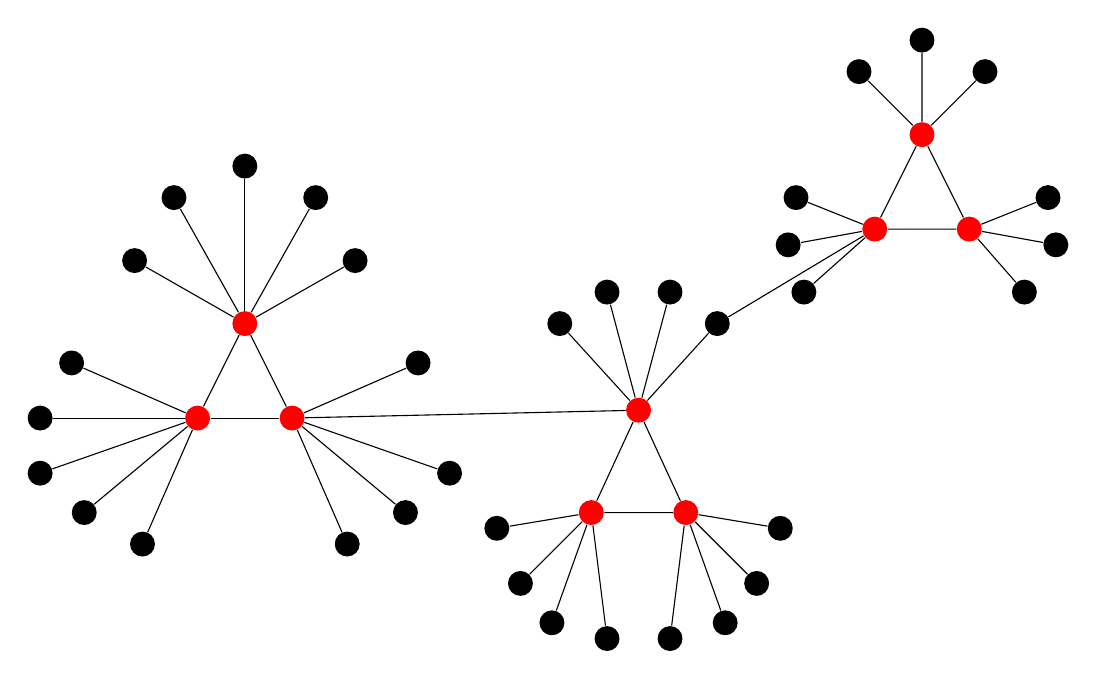
\begin{tikzpicture}[scale=0.4]

\tikzstyle{vertex}=[circle,fill=black,minimum size=9pt,inner sep=0pt]
\node[vertex, fill=red] (1) at (1.5,3){};
\node[vertex, fill=red] (2) at (0,0){};
\node[vertex, fill=red] (3) at (3,0){};

\node[vertex] (4) at (-2,5){};
\node[vertex] (5) at (-0.75,7){};
\node[vertex] (6) at (1.5,8){};
\node[vertex] (7) at (3.75,7){};
\node[vertex] (8) at (5,5){};

\node[vertex] (9) at (7,1.75){};
\node[vertex, fill=red] (10) at (14,0.25){};
\node[vertex] (11) at (4.75,-4){};
\node[vertex] (12) at (6.6,-3){};
\node[vertex] (13) at (8,-1.75){};

\node[vertex] (14) at (-4,1.75){};
\node[vertex] (15) at (-5,0){};
\node[vertex] (16) at (-1.75,-4){};
\node[vertex] (17) at (-3.6,-3){};
\node[vertex] (18) at (-5,-1.75){};

\node[vertex, fill=red] (19) at (12.5,-3){};
\node[vertex, fill=red] (20) at (15.5,-3){};

\node[vertex] (21) at (9.5,-3.5){};
\node[vertex] (22) at (10.25,-5.25){};
\node[vertex] (23) at (11.25,-6.5){};
\node[vertex] (24) at (13,-7){};

\node[vertex] (25) at (18.5,-3.5){};
\node[vertex] (26) at (17.75,-5.25){};
\node[vertex] (27) at (16.75,-6.5){};
\node[vertex] (28) at (15,-7){};

\node[vertex] (29) at (11.5,3){};
\node[vertex] (30) at (13,4){};
\node[vertex] (31) at (15,4){};
\node[vertex] (32) at (16.5,3){};

\node[vertex, fill=red] (33) at (21.5,6){};
\node[vertex, fill=red] (34) at (24.5,6){};
\node[vertex, fill=red] (35) at (23,9){};

\node[vertex] (36) at (23,12){};
\node[vertex] (37) at (25,11){};
\node[vertex] (38) at (21,11){};

\node[vertex] (39) at (19,7){};
\node[vertex] (40) at (18.75,5.5){};
\node[vertex] (41) at (19.25,4){};

\node[vertex] (42) at (27,7){};
\node[vertex] (43) at (27.25,5.5){};
\node[vertex] (44) at (26.25,4){};

\draw (33) -- (34)node[draw=none,fill=none,near end,right,font=\tiny] {};
\draw (33) -- (35)node[draw=none,fill=none,near end,right,font=\tiny] {};
\draw (35) -- (34)node[draw=none,fill=none,near end,right,font=\tiny] {};

\draw (33) -- (39)node[draw=none,fill=none,near end,right,font=\tiny] {};
\draw (33) -- (40)node[draw=none,fill=none,near end,right,font=\tiny] {};
\draw (33) -- (41)node[draw=none,fill=none,near end,right,font=\tiny] {};

\draw (34) -- (42)node[draw=none,fill=none,near end,right,font=\tiny] {};
\draw (34) -- (43)node[draw=none,fill=none,near end,right,font=\tiny] {};
\draw (34) -- (44)node[draw=none,fill=none,near end,right,font=\tiny] {};

\draw (35) -- (36)node[draw=none,fill=none,near end,right,font=\tiny] {};
\draw (35) -- (37)node[draw=none,fill=none,near end,right,font=\tiny] {};
\draw (35) -- (38)node[draw=none,fill=none,near end,right,font=\tiny] {};

\draw (33) -- (32)node[draw=none,fill=none,near end,right,font=\tiny] {};

\draw (10) -- (20)node[draw=none,fill=none,near end,right,font=\tiny] {};
\draw (10) -- (19)node[draw=none,fill=none,near end,right,font=\tiny] {};
\draw (20) -- (19)node[draw=none,fill=none,near end,right,font=\tiny] {};

\draw (19) -- (21)node[draw=none,fill=none,near end,right,font=\tiny] {};
\draw (19) -- (22)node[draw=none,fill=none,near end,right,font=\tiny] {};
\draw (19) -- (23)node[draw=none,fill=none,near end,right,font=\tiny] {};
\draw (19) -- (24)node[draw=none,fill=none,near end,right,font=\tiny] {};

\draw (20) -- (25)node[draw=none,fill=none,near end,right,font=\tiny] {};
\draw (20) -- (26)node[draw=none,fill=none,near end,right,font=\tiny] {};
\draw (20) -- (27)node[draw=none,fill=none,near end,right,font=\tiny] {};
\draw (20) -- (28)node[draw=none,fill=none,near end,right,font=\tiny] {};

\draw (10) -- (29)node[draw=none,fill=none,near end,right,font=\tiny] {};
\draw (10) -- (30)node[draw=none,fill=none,near end,right,font=\tiny] {};
\draw (10) -- (31)node[draw=none,fill=none,near end,right,font=\tiny] {};
\draw (10) -- (32)node[draw=none,fill=none,near end,right,font=\tiny] {};

\draw (1) -- (2)node[draw=none,fill=none,near end,right,font=\tiny] {};
\draw (2) -- (3)node[draw=none,fill=none,near end,left,font=\tiny] {};
\draw (1) -- (3)node[draw=none,fill=none,near end,left,font=\tiny] {};
\draw (1) -- (4)node[draw=none,fill=none,near end,left,font=\tiny] {};
\draw (1) -- (5)node[draw=none,fill=none,near end,left,font=\tiny] {};
\draw (1) -- (6)node[draw=none,fill=none,near end,left,font=\tiny] {};
\draw (1) -- (7)node[draw=none,fill=none,near end,left,font=\tiny] {};
\draw (1) -- (8)node[draw=none,fill=none,near end,left,font=\tiny] {};

\draw (3) -- (9)node[draw=none,fill=none,near end,left,font=\tiny] {};
\draw (3) -- (10)node[draw=none,fill=none,near end,left,font=\tiny] {};
\draw (3) -- (11)node[draw=none,fill=none,near end,left,font=\tiny] {};
\draw (3) -- (12)node[draw=none,fill=none,near end,left,font=\tiny] {};
\draw (3) -- (13)node[draw=none,fill=none,near end,left,font=\tiny] {};

\draw (2) -- (14)node[draw=none,fill=none,near end,left,font=\tiny] {};
\draw (2) -- (15)node[draw=none,fill=none,near end,left,font=\tiny] {};
\draw (2) -- (16)node[draw=none,fill=none,near end,left,font=\tiny] {};
\draw (2)-- (17)node[draw=none,fill=none,near end,left,font=\tiny] {};
\draw (2) -- (18)node[draw=none,fill=none,near end,left,font=\tiny] {};
%\path[-]          (0)  edge   [bend right, left,midway, font=\tiny]   node {$3$} (1);
%\path[-]          (0)  edge   [bend left, right,midway, font=\tiny]   node {$4$} (2);
\end{tikzpicture}
\caption{all nodes in the graph are adjacent to one of three triangles}
\end{figure}
\section{Solution and Analysis}
To test how well the presented method is suitable to find the average connectivity of triangles in a graph I will first generate a graph with $\tau$ triangles. For each triangle I draw a random number $r$ between 1 and $a$ and assign each node of the triangle $r$ adjacent nodes (thus this triangle gets $3\times r$ adjacent nodes). All in all the generated graph consists of only triangles, where each triangle gets a random number of adjacent nodes that are equally distributed among the triangle nodes. Next I shuffle the order of the edges to generate a graph stream in which the edges appear in random order. Now I use the \textit{Neighborhood Sampling} method to sample triangles from this stream where I use choose $e$ estimators. As described in the paper each estimator can either hold a triangle or not. For the case that an estimator is holding a triangle we take this triangle into our sample with probability $\frac{c}{2\Delta}$ ($c$ is the number of edges the	 estimator observed that are adjacent to the first edge of the triangle that arrived in the stream and $\Delta$ is the maximum degree of a node in the graph). For each triangle that I get in my sample I estimate the total number of adjacent nodes as described in 3.1. Finally I compare the mean and variance of the \textit{connectivity} that I got from my sample with the actual mean and variance of the triangle population.

The sampling method is simple random sampling with replacement. Therefore I expect that I get an unbiased estimator for the overall \textit{connectivity} of the triangles. The size of the samples that the method allows me to draw depends both on the number of estimators and the maximum degree $\Delta$ in the generated graph. My estimation should get more accurate the higher I choose the number of estimators $e$ as more estimators return a larger sample. At the same time my estimation should become less accurate, the larger I choose $a$ because a larger $a$ results in a larger value $\Delta$ which decreases the size of the sample I can draw from the estimators.

\subsection{Estimating the number of adjacent nodes of a triangle}
The estimators from which the triangles are being sampled are first sampling a random edge $r_1$ from the stream, then they sample a random edge $r_2$ from the substream of edges that arrive after $r_1$ and are adjacent to it. Finally they sample an edge $r_3$ that closes the wedge $r_1r_2$ and forms the triangle $r_1r_2r_3$. Each estimator keeps track of the number of edges it observes that are adjacent to $r_1$ and arrive after it in the stream. This number is kept in a counter $c$. Thus $c$ keeps track of the number of edges that arrive after $r_1$ and which are adjacent to either of two nodes of the triangle (the two nodes of the triangle that are connected by $r_1$). For each estimator that is returning a triangle into my sample I estimate the total number of adjacent nodes to this triangle as $((c-2)\frac{4}{3})\times\frac{3}{2}$. The term $(c-2)$ is the number of $r_1$-adjacent edges that were observed in the stream after $r_1$ excluding the two edges that belong to the triangle ($r_2$ and $r_3$). The term $(c-2)\frac{4}{3}$ represents the $(c-2)$ edges that are adjacent to $r_1$ and arrived after $r_1$ in the stream \textit{plus} the expected number of edges that arrived in the stream before $r_1$ (the expected number of $r_1$ adjacent edges that arrived before $r_1$ is $\frac{1}{3}(c-2)$). Thus the term $((c-2)\frac{4}{3})$ represents the number of edges that are adjacent to the $r_1$ edge of the triangle. The edge $r_1$ represents two nodes of the triangle. My estimate for the number of edges that are adjacent to the third node of the triangle is $\frac{1}{2}((c-2)\frac{4}{3})$, because I am assuming that the number of adjacent nodes are equally distributed among the three triangle nodes. The total number of adjacent edges to this triangle is then $((c-2)\frac{4}{3})\times\frac{3}{2}$.
\section{Experimental Results}
\subsection{Method Implementation}
First I implemented the method from the paper and verified that my implementation is correct by reproducing the experiments from the paper with the same datasets which I downloaded from https://snap.stanford.edu/data. To verify my implementation I downloaded the amazon, dblp and livejournal graphs and got similar results as the authors of the paper. Further I downloaded a Protein-Protein-Interaction Network from http://thebiogrid.org/ and ran the method on this dataset. In addition to the number of triangles that was estimated by the method, I noted the number of triangles that I was able to sample from the chosen number of estimators as listed in Table 1. 
\subsection{Testing of the method on simulated graphs}
I tested the method for triangle sampling with the following parameters for $\tau$ (number of generated triangles), $a$ (maximum number of adjacent nodes that gets assigned to a triangle node) and $e$ (number of estimators from which we sample the triangles). In Table 2 $\mu$ lists the mean \textit{connectivity} of the generated triangles and $v$ lists the \textit{connectivity}-variance of the generated triangles for the chosen parameters $\tau$ and $a$. In the table cells, $s$ lists the sample size that I got from the $e$ estimators and 
$\mu_{est}, var_{est}$ list the mean and variance of \textit{connectivity} I got from my sample.
\begin{center}
\begin{table}
\resizebox{\textwidth}{!}{
\begin{tabular}{l|c|c|c}
$\tau, a \Rightarrow \mu, v$ &$e=10000$&$e=100000$&$e=1000000$\\
\hline 
500, 10 $\Rightarrow$ 16, 115 & $s=21, \mu_{est}=16 ,var_{est}=119$ & $s=204, \mu_{est}=14, var_{est}=99$&  $s=2273, \mu_{est}=16, var_{est}=105$\\
500, 30 $\Rightarrow$ 46, 962 & $s=2, \mu_{est}=20 ,var_{est}=360$ & $s=35, \mu_{est}=46, var_{est}=936$&  $s=302, \mu_{est}=44, var_{est}=939$\\
500, 50 $\Rightarrow$ 76, 2633 & $s=1, \mu_{est}=91 ,var_{est}=0$ & $s=11, \mu_{est}=57, var_{est}=2129$&  $s=124, \mu_{est}=79, var_{est}=2841$\\
500, 100 $\Rightarrow$ 152, 10576 & $s=0, \mu_{est}=\emptyset ,var_{est}=\emptyset$ & $s=2, \mu_{est}=112, var_{est}=6210$&  $s=30, \mu_{est}=158, var_{est}=9290$\\
1000, 10 $\Rightarrow$ 16, 116 & $s=18, \mu_{est}=15 ,var_{est}=72$ & $s=196, \mu_{est}=15, var_{est}=90$&  $s=2157, \mu_{est}=15, var_{est}=100$\\
1000, 30$\Rightarrow$ 45, 959 & $s=5, \mu_{est}=68 ,var_{est}=647$ & $s=31, \mu_{est}=46, var_{est}=766$&  $s=311, \mu_{est}=43, var_{est}=776$\\
1000, 50$\Rightarrow$ 76, 2757 & $s=1, \mu_{est}=19 ,var_{est}=0$ & $s=15, \mu_{est}=78, var_{est}=1903$&  $s=133, \mu_{est}=74, var_{est}=2388$\\
1000, 100$\Rightarrow$ 155, 11478 & $s=0, \mu_{est}=\emptyset ,var_{est}=\emptyset$ & $s=2, \mu_{est}=323, var_{est}=573$&  $s=36, \mu_{est}=150, var_{est}=9374$\\
2000, 10$\Rightarrow$ 16, 118 & $s=27, \mu_{est}=19, var_{est}=75$ & $s=223, \mu_{est}=16, var_{est}=106$&  $s=2078, \mu_{est}=15, var_{est}=99$\\
2000, 30$\Rightarrow$ 46, 996 & $s=2, \mu_{est}=55 ,var_{est}=1437$ & $s=29, \mu_{est}=39, var_{est}=940$&  $s=323, \mu_{est}=42, var_{est}=762$\\
2000, 50$\Rightarrow$ 76, 2766 & $s=1, \mu_{est}=7 ,var_{est}=0$ & $s=16, \mu_{est}=82, var_{est}=1710$&  $s=131, \mu_{est}=79, var_{est}=2614$\\
2000, 100$\Rightarrow$ 150, 10605& $s=0, \mu_{est}=\emptyset ,var_{est}=\emptyset$ & $s=2, \mu_{est}=69, var_{est}=255$&  $s=28, \mu_{est}=155, var_{est}=7854$\\
\end{tabular}
}
\caption{This table lists my experiment results. It can be read as follows: The first column lists the propoerties of the generated graphs. The column entry $1000, 50 \Rightarrow 76,2757$ means I generated a graph that consists of 1000 triangles where for each triangle $t$ I draw a number $r$ between 1 and 50 and assigned each node of $t$ $r$ adjacent nodes. The mean \textit{connectivity} of the triangles in this graph was 76 and the variance of the \textit{connectivity} was 2757. Then I used $10^3$,$10^4$ and $10^5$ estimators to sample triangles from this graph. For $10^4$ estimators for example I could draw $s=15$ triangles into my sample. For each of these triangles I estimated the total number of adjacent nodes as explained in 3.1. Finally I computed the mean and variance \textit{connectivity} of my sample as $\mu_{est}$ and $var_{est}$.}
\end{table}
\end{center}
\section{Conclusion and Discussion}
0.5 page
\end{document}